\documentclass[a4paper,12pt,singlespacing]{article}
% \usepackage[left=2.5cm,right=2.5cm,top=2.5cm]{geometry}
\usepackage{titlesec}
\usepackage{setspace}
\usepackage[utf8]{inputenc}
\usepackage{graphicx}
\usepackage{color}
\usepackage[hidelinks]{hyperref}
\usepackage[style=ieee, sorting=none]{biblatex}
\usepackage[english]{babel}
\usepackage{tikz}
\usepackage{pgfplots}
\usepackage{float}
\usepackage{listings,xcolor}
\usepackage{caption}
\usepackage[acronym]{glossaries}
\makeglossaries
\addbibresource{sample.bib}

% Abstände definieren
\titlespacing*{\section}{0pt}{35pt}{35pt}
\titlespacing*{\subsection}{0pt}{20pt}{20pt}
\titlespacing*{\subsubsection}{0pt}{10pt}{10pt}

\begin{document}
\selectlanguage{english}
% Absatzeinrückung verhindern
\setlength{\parindent}{0ex}

\begin{titlepage}
	
		%----------------------------------------------------------------------------------------
	%	LOGO SECTION
	%----------------------------------------------------------------------------------------
	
	\begin{minipage}{0.4\textwidth}
		\begin{flushleft} \large
			
\includegraphics[width=3.5cm]{./Images/conti_logo.png} % Include a department/university logo - this will require the graphicx package
		\end{flushleft}
	\end{minipage}
	~
	\begin{minipage}{0.5\textwidth}
		\begin{flushright} \large
			
\includegraphics[width=7cm]{./Images/logo.png} % Include a department/university logo - this will require the graphicx package
		\end{flushright}
	\end{minipage}\\[1.5cm]
	
	%----------------------------------------------------------------------------------------
	
	\newcommand{\HRule}{\rule{\linewidth}{0.5mm}} % Defines a new command for the horizontal lines, change thickness here
	
	\center % Center everything on the page
	
	%----------------------------------------------------------------------------------------
	%	HEADING SECTIONS
	%----------------------------------------------------------------------------------------
	
	\textsc{\LARGE Ravensburg Weingarten University}\\[1cm] % Name of your university/college
	\textsc{\large  \textbf{Bachelor Thesis}}\\[0.5cm] % Minor heading such as course title
	
	%----------------------------------------------------------------------------------------
	%	TITLE SECTION
	%----------------------------------------------------------------------------------------
	
	\HRule \\[0.4cm]
	{ \huge \bfseries Development of a System Testing Framework for eCAL-Based Inter-Process-Communication}\\[0.4cm] % Title of your document
	\HRule \\[1.5cm]
	
	%----------------------------------------------------------------------------------------
	%	AUTHOR SECTION
	%----------------------------------------------------------------------------------------
	
	\begin{minipage}{0.5\textwidth}
		\begin{flushleft}\fontsize{11pt}{14pt}\selectfont
		\textbf{Author:} Emircan Tutar\\[4pt]
		\textbf{Address:} Heyderstr. 7\\[4pt]
		\textbf{City:} 88131 Lindau\\[7pt]
		\textbf{Student ID:} 35606\\[4pt]
		\textbf{Program:} Applied Computer Science\\[4pt]
		\end{flushleft}
	\end{minipage}
	~
	\begin{minipage}{0.45\textwidth}
		\begin{flushleft} \fontsize{11pt}{14pt}\selectfont
		\textbf{1st Supervisor:} \\[2pt]
		Prof. Dr. Marius Hofmeister \\
		Ravensburg Weingarten University \\[10pt]
		\textbf{2nd Supervisor:} \\[2pt]
		M.Sc. Kerstin Keller \\
		Continental\\[7pt]
		\end{flushleft}
	\end{minipage}\\[3cm]
	
	%----------------------------------------------------------------------------------------
	%	DATE SECTION
	%----------------------------------------------------------------------------------------
	
	{\large \today}\\[0cm] % Date, change the \today to a set date if you want to be precise
	
	\vfill % Fill the rest of the page with whitespace
	
\end{titlepage}

\pagebreak
\vspace*{2cm}
 \textit{Current software development demands quick solutions to fulfill constantly changing requirements. Distributed systems, where software processes run on separate computing nodes and communicate with each other, have become increasingly important. To enable effective communication within such systems, inter-process communication (IPC) frameworks like the enhanced Communication Abstraction Layer (eCAL) are commonly used. eCAL allows data to be exchanged rapidly and reliably, enabling faster implementation of new features and adjustments within complex software projects. } \\ 

 \textit{As these systems grow in complexity, ensuring software quality becomes more challenging but also more critical. Failures or errors in communication middleware can lead to significant problems, especially in areas like automotive or robotics, where safety and reliability are essential. Thus, the central question arises: how can the reliability and correctness of eCAL-based IPC systems be systematically ensured? The goal of this thesis is to develop and evaluate a structured system testing framework specifically tailored for eCAL-based communication, aiming to detect faults early and increase overall software quality. } \\ 

 \textit{To achieve this goal, various system testing approaches will be analyzed and adapted for eCAL. This includes evaluating unit tests, integration tests, and system-level testing methods. Additionally, automation and continuous testing techniques within CI/CD pipelines will be considered. A concrete example implementation of these test strategies will be demonstrated, evaluated, and compared to ensure practical applicability and effectiveness. }

\pagebreak

\tableofcontents
\pagebreak

% List of Figures
\listoffigures
\addcontentsline{toc}{section}{List of Figures}
\pagebreak

% List of Listings
\lstlistoflistings
\addcontentsline{toc}{section}{List of Listings}
\pagebreak

\section*{List of Abbreviations}
\addcontentsline{toc}{section}{List of Abbreviations}

\begin{tabbing}
	XXXXXXXXX \= XXXXXXXXXXXXXXXXXXXXXXXXXXX \kill %length
	\textbf{IPC} \> Inter-Process Communication\\[0.5cm]
	\textbf{eCAL} \> enhanced Communication Abstraction Layer\\[0.5cm]
	\textbf{CI/CD} \> Continuous Integration / Continuous Delivery\\[0.5cm]
	\textbf{RPC} \> Remote Procedure Call\\[0.5cm]
	\textbf{IoT} \> Internet of Things\\[0.5cm]
\end{tabbing}

\pagebreak

\selectlanguage{english}
\clearpage

\section{Einleitung}
Dies ist eine beispielhafte Quelle~\cite{example2024}.

\subsection{Motivation}

\subsection{Problemstellung}


\subsection{Zielsetzung}



\selectlanguage{english}
\clearpage
\section{Theoretical Foundations}

In this chapter, the theoretical background necessary to understand the development of a system testing framework for eCAL is presented. Section 2.1 introduces the concept of distributed systems, including their characteristics and common use cases. Section 2.2 explains the fundamentals of inter-process communication (IPC) and highlights different communication mechanisms. In Section 2.3, the role of middleware in distributed environments is discussed, with a focus on commonly used solutions such as ROS, DDS, and eCAL. Section 2.4 gives a detailed overview of the eCAL framework, including its architecture, features, and typical applications. Section 2.5 provides essential concepts in software testing, such as test levels, types, and techniques. Finally, Section 2.6 outlines specific challenges in testing middleware systems, presents current testing approaches, and analyzes the limitations of testing practices in the context of eCAL.

\subsection{Distributed Systems}

\subsubsection{Definition and Concepts}

A distributed system is a network of independent computers that appears to users as a single coherent system. In distributed systems, multiple computing devices communicate and coordinate their activities by passing messages to achieve a common goal \cite{tanenbaum2017}. Such systems consist of independent components located on different networked computers, which interact with each other by exchanging messages.
\\
\\
The primary goal of distributed systems is to share resources, increase performance, and provide reliable and fault-tolerant operations. Resources such as processing power, memory, storage, and data can be shared between multiple nodes within the system, enhancing system efficiency and scalability \cite{coulouris2012}.

Figure~\ref{fig:distributed_architecture} illustrates a basic distributed system consisting of multiple independent nodes communicating over a network. Each node may serve a specific role, such as providing services, accessing shared resources, or coordinating tasks.

\begin{figure}[H]
	\centering
	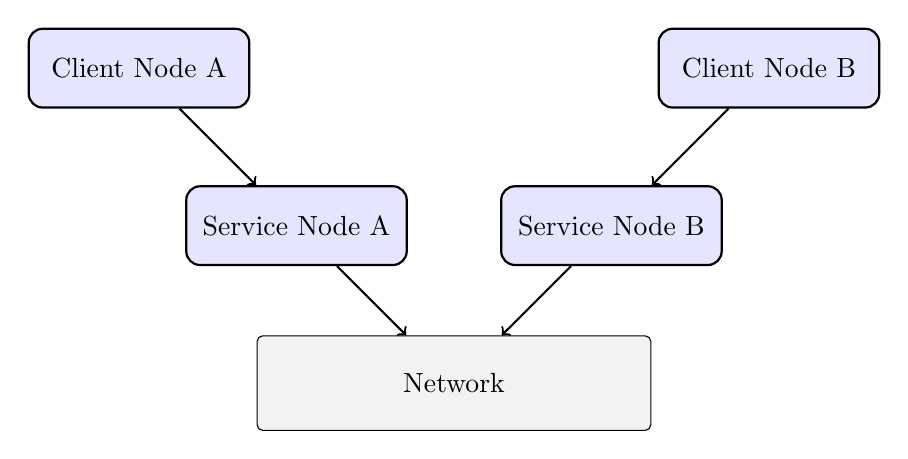
\begin{tikzpicture}[
		node/.style={draw, thick, minimum width=2.8cm, minimum height=1cm, rounded corners=5pt, fill=blue!10},
		conn/.style={->, thick},
		network/.style={draw, fill=gray!10, rounded corners=2pt}
		]
		
		% Nodes
		\node[node] (client1) at (-4, 2) {Client Node A};
		\node[node] (client2) at (4, 2) {Client Node B};
		\node[node] (server1) at (-2, 0) {Service Node A};
		\node[node] (server2) at (2, 0) {Service Node B};
		
		% Network Cloud
		\node[network, minimum width=5cm, minimum height=1.2cm] (network) at (0,-2) {Network};
		
		% Arrows from Clients to Services
		\draw[conn] (client1) -- (server1);
		\draw[conn] (client2) -- (server2);
		
		% Arrows from Services to Network
		\draw[conn] (server1) -- (network);
		\draw[conn] (server2) -- (network);
		
	\end{tikzpicture}
	\caption{Basic architecture of a distributed system with multiple clients and services connected through a network}
	\label{fig:distributed_architecture}
\end{figure}


\subsubsection{Characteristics and Challenges}

Distributed systems have several key characteristics, including concurrency, scalability, transparency, and fault tolerance. Concurrency refers to multiple processes executing simultaneously. Scalability describes the capability of the system to grow easily in size and workload. Transparency ensures the complexity of the system remains hidden from users, providing an impression of a single unified system. Fault tolerance describes the system's capability to continue operation even when individual components fail \cite{tanenbaum2017}.
\\
\\
However, developing and managing distributed systems can be challenging. Problems related to communication delays, synchronization between processes, security, and managing the complexity of the overall system must be addressed effectively to ensure reliable operations \cite{coulouris2012}.

\subsubsection{Application Areas}

Distributed systems are widely used across many industries. In automotive systems, they support advanced driver-assistance systems (ADAS), autonomous driving, and vehicle communication systems. Robotics heavily relies on distributed systems for complex coordination tasks, such as collaborative robotics, autonomous navigation, and real-time control. The Internet of Things (IoT) is another prominent application area, where distributed systems enable efficient communication between countless smart devices and sensors, facilitating smart homes, smart cities, and industrial automation \cite{tanenbaum2017,coulouris2012}.





\subsection{Inter-Process Communication (IPC)}

\subsubsection{Overview and Importance}

Inter-process communication (IPC) refers to mechanisms that allow processes to communicate and exchange data. IPC is a crucial component in distributed and concurrent systems, enabling different software processes running on one or multiple computers to coordinate and share information effectively \cite{stallings2018}. Effective IPC mechanisms are essential for ensuring the smooth and reliable functioning of complex software systems, especially in critical applications such as automotive control systems, robotics, and industrial automation \cite{tanenbaum2015}.

\subsubsection{Common IPC Mechanisms}

There are several commonly used IPC mechanisms, each suitable for different scenarios and requirements. The most frequently used methods include shared memory, message passing, and remote procedure calls (RPC) \cite{stallings2018,tanenbaum2015}.
\\
\\

Figure~\ref{fig:ipc_methods} illustrates a simplified comparison of common inter-process communication mechanisms. Shared memory allows processes to access a common memory region directly. Message passing transfers data through explicit send/receive actions. Remote Procedure Call (RPC) abstracts communication by allowing a process to call functions in another process as if they were local.

\begin{figure}[H]
	\centering
	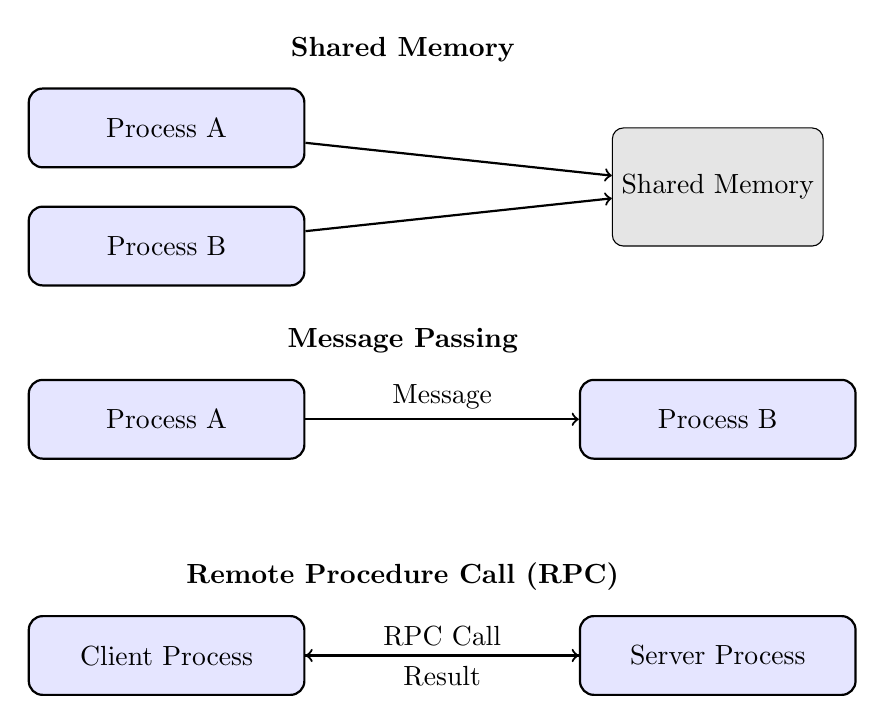
\begin{tikzpicture}[
		node/.style={draw, thick, minimum width=3.5cm, minimum height=1cm, rounded corners=5pt, fill=blue!10},
		conn/.style={->, thick},
		label/.style={font=\bfseries, align=center}
		]
		
		% Shared Memory
		\node[label] at (0,8) {Shared Memory};
		\node[node] (shmA) at (-3,7) {Process A};
		\node[node] (shmB) at (-3,5.5) {Process B};
		\node[draw, fill=gray!20, minimum width=2.5cm, minimum height=1.5cm, rounded corners=4pt] at (4,6.25) (shm) {Shared Memory};
		\draw[conn] (shmA) -- (shm);
		\draw[conn] (shmB) -- (shm);
		
		% Message Passing
		\node[label] at (0,4.3) {Message Passing};
		\node[node] (msgA) at (-3,3.3) {Process A};
		\node[node] (msgB) at (4,3.3) {Process B};
		\draw[conn] (msgA) -- node[above] {Message} (msgB);
		
		% RPC
		\node[label] at (0,1.3) {Remote Procedure Call (RPC)};
		\node[node] (rpcClient) at (-3,0.3) {Client Process};
		\node[node] (rpcServer) at (4,0.3) {Server Process};
		\draw[conn] (rpcClient) -- node[above] {RPC Call} (rpcServer);
		\draw[conn] (rpcServer) -- node[below] {Result} (rpcClient);
		
	\end{tikzpicture}
	\caption{Comparison of common IPC mechanisms: Shared Memory, Message Passing, and Remote Procedure Call (RPC)}
	\label{fig:ipc_methods}
\end{figure}


\textbf{Shared Memory:}

Shared memory is one of the fastest IPC methods, allowing processes to communicate directly by accessing a common area of memory. Processes write and read data directly into this shared space, avoiding the overhead of explicit communication. However, managing synchronization and ensuring data integrity can become challenging and requires careful implementation of synchronization methods, such as semaphores or mutexes \cite{stallings2018, ipc_performance_analysis}.
\\
\\
\textbf{Message Passing:}

Message passing involves processes communicating through messages. This approach ensures a clear separation between processes, providing safer communication. Messages are sent explicitly from one process to another using defined communication channels, such as pipes or sockets. While message passing typically has higher overhead compared to shared memory, it is easier to manage synchronization, and it allows better scalability in distributed environments \cite{tanenbaum2015}.
\\
\\
\textbf{Remote Procedure Calls (RPC):}

Remote Procedure Calls (RPC) enable processes to invoke procedures or functions on remote systems as if they were local calls. RPC abstracts network communication, making distributed system interactions easier to develop and maintain. RPC is widely used in distributed applications and middleware solutions due to its simplicity and clear programming model, despite some performance overhead from serialization and network transmission \cite{coulouris2012}.

\subsubsection{Zero-Copy Communication}

Zero-copy communication is an advanced IPC technique designed to minimize unnecessary data copying between processes. Traditional communication methods often involve copying data multiple times, significantly reducing performance and increasing latency. Zero-copy mechanisms avoid this overhead by allowing direct data transfers between processes, usually through shared memory or specialized network interfaces. By reducing the number of data copies, zero-copy significantly enhances performance and efficiency in systems with high throughput and low latency requirements, such as high-performance computing or real-time systems \cite{raiciu2017}.




\subsection{Middleware in Distributed Systems}

\subsubsection{Definition and Role of Middleware}

Middleware is software that sits between applications and the underlying operating system or network infrastructure, enabling easier communication and coordination within distributed systems. Its main role is to simplify development by abstracting complexities associated with networked and distributed computing, such as communication protocols, data exchange, and interoperability between diverse systems \cite{bernstein1996}. Middleware allows software developers to focus more on the application logic rather than the low-level communication and network details.

\subsubsection{Common Middleware Solutions}

Various middleware technologies are available today, each designed to address specific communication and coordination needs. 
Some widely used middleware solutions include the Robot Operating System (ROS) \cite{quigley2009}, the Data Distribution Service (DDS) \cite{pardo2003}, and the enhanced Communication Abstraction Layer (eCAL) \cite{ecal_official_docs}.
\\
\\
\textbf{Robot Operating System (ROS):}

ROS is an open-source middleware widely used in robotics. It provides a structured communication framework that includes services like message passing, data visualization, hardware abstraction, and numerous tools for robotics development. ROS simplifies building complex robotic systems by offering standardized communication interfaces and extensive community-supported tools and libraries \cite{quigley2009}.
\\
\\
\textbf{Data Distribution Service (DDS):}

DDS is a standardized middleware designed primarily for real-time and high-performance distributed applications. It employs a publisher-subscriber communication model, where components communicate by exchanging messages without direct connections between producers and consumers. DDS provides reliable and scalable communication, making it suitable for critical applications such as automotive systems, aerospace, industrial automation, and healthcare \cite{pardo2003}.
\\
\\
\textbf{enhanced Communication Abstraction Layer (eCAL):}

eCAL is a middleware specifically designed for efficient inter-process communication (IPC) in distributed environments. It offers high-speed message exchange, remote procedure calls (RPC), and shared memory communication. eCAL's lightweight nature and focus on performance make it ideal for scenarios that require fast data transfer, such as automotive software systems, industrial automation, and complex IoT solutions \cite{ecal_github}.
\\
\begin{table}[H]
	\centering
	\renewcommand{\arraystretch}{1.5}
	\begin{tabular}{|p{2.25cm}|p{3.22cm}|p{3.22cm}|p{3.22cm}|}
		\hline
		\textbf{Layer} & \textbf{ROS} & \textbf{DDS} & \textbf{eCAL} \\
		\hline
		Application Layer & User Applications & User Applications & User Applications \\
		\hline
		Middleware API & rospy, roscpp & DDS API & eCAL API (C++, Python, etc.) \\
		\hline
		Core-Components & ROS-Master, Topics, Services & RTPS Protocol & Pub/Sub, RPC \\
		\hline
		Transport Layer & TCP-ROS, UDP-ROS & UDP/IP & Shared-Memory, UDP, TCP \\
		\hline
		Operating System & Linux, Windows, macOS & OS-dependent & Linux, Windows \\
		\hline
	\end{tabular}
	\caption{Architecture comparison between ROS, DDS, and eCAL middleware}
	\label{tab:middleware_comparison}
\end{table}

Table~\ref{tab:middleware_comparison} presents a layered architecture comparison between ROS, DDS, and eCAL. Each middleware abstracts the communication stack differently, but all provide core functionality for distributed system communication.
\\

\subsubsection{Benefits and Challenges of Middleware}

Middleware plays a crucial role in distributed systems by abstracting the complexity of communication between software components. It enables interoperability between heterogeneous systems, promotes modular design, and supports scalability by decoupling application logic from low-level infrastructure details \cite{josuttis2007, coulouris2012}. Through standardized interfaces and reusable communication patterns, middleware simplifies the integration of new components and accelerates system development.
\\
\\
However, the use of middleware also introduces several challenges. The additional abstraction layers can lead to performance overhead, making it more difficult to meet strict real-time requirements. Furthermore, debugging and testing become more complex due to the increased system opacity introduced by middleware components \cite{josuttis2007, coulouris2012}. Therefore, when choosing middleware, it is important to consider both its advantages and the limitations it may introduce to the overall system architecture.





\subsection{eCAL Framework}

\subsubsection{Overview and Architecture}

The enhanced Communication Abstraction Layer (eCAL) is an open-source middleware designed specifically for efficient inter-process communication (IPC) in distributed environments. It simplifies the exchange of data between processes running on the same device or across multiple networked computers. eCAL uses a decentralized publish-subscribe architecture, allowing multiple processes to communicate directly without relying on a central broker \cite{ecal_github}.
\\
\\
eCAL has a modular and flexible architecture. It supports multiple transport layers, including shared memory for communication between processes on the same machine and TCP or UDP for communication over networks. This adaptive approach ensures optimal performance by automatically selecting the best available communication method based on the system's environment and requirements \cite{ecal_official_docs}.
\\
\\
Figure~\ref{fig:ecal_architecture} illustrates the basic eCAL architecture. It shows how multiple publisher and subscriber nodes communicate over topics. Additionally, a monitoring component observes the activity of each node to support debugging and analysis.
\\
\begin{figure}[H]
	\centering
	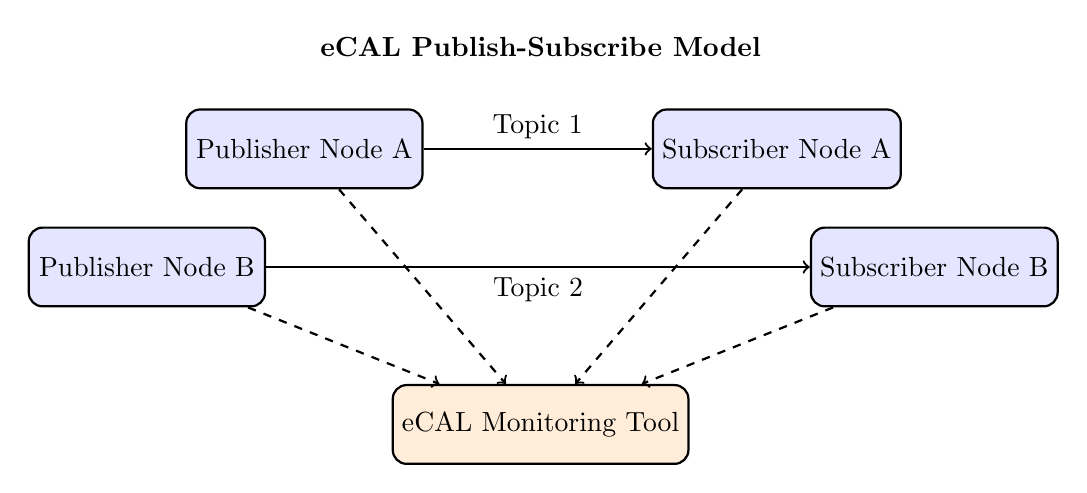
\begin{tikzpicture}[
		component/.style={draw, thick, minimum width=3cm, minimum height=1cm, rounded corners=5pt, fill=blue!10},
		arrow/.style={->, thick}
		]
		
		% Nodes
		\node[component] (pub1) at (0,2.5) {Publisher Node A};
		\node[component] (pub2) at (-2,1) {Publisher Node B};
		\node[component] (sub1) at (6,2.5) {Subscriber Node A};
		\node[component] (sub2) at (8,1) {Subscriber Node B};
		\node[component, fill=orange!15] (monitor) at (3,-1) {eCAL Monitoring Tool};
		
		% Arrows
		\draw[arrow] (pub1) -- node[above] {Topic 1} (sub1);
		\draw[arrow] (pub2) -- node[below] {Topic 2} (sub2);
		\draw[arrow, dashed] (pub1) -- (monitor);
		\draw[arrow, dashed] (pub2) -- (monitor);
		\draw[arrow, dashed] (sub1) -- (monitor);
		\draw[arrow, dashed] (sub2) -- (monitor);
		
		% Labels
		\node at (3,3.8) {\textbf{eCAL Publish-Subscribe Model}};
		
	\end{tikzpicture}
	\caption{Simplified architecture of the eCAL framework with publisher, subscriber, and monitoring components}
	\label{fig:ecal_architecture}
\end{figure}

\subsubsection{Core Features}

eCAL provides several important features which make it suitable for a wide range of applications:
\\
\\
- \textbf{High Performance:} eCAL achieves very low latency and high throughput through optimized data transport methods, including zero-copy shared memory communication. This makes it ideal for real-time and performance-critical systems \cite{ecal_github,ecal_official_docs}.
\\
\\
- \textbf{Multi-Language Support:} eCAL offers interfaces for several programming languages such as C++, C\#, Python, Java, and Go, enabling easy integration into various software projects \cite{ecal_official_docs}.
\\
\\
- \textbf{Cross-Platform Compatibility:} eCAL supports multiple platforms, including Windows, Linux, and macOS. This compatibility allows easy deployment in diverse environments and distributed systems \cite{ecal_official_docs}.
\\
\\
- \textbf{Built-in Tools and Monitoring:} eCAL includes tools for visualizing, recording, replaying, and monitoring inter-process communication. These tools assist developers in debugging, performance analysis, and overall system reliability \cite{ecal_github,ecal_official_docs}.

\subsubsection{Applications and Use Cases}

Due to its efficiency and reliability, eCAL is widely used in industries that demand robust real-time communication. For example, in automotive applications, eCAL supports advanced driver-assistance systems (ADAS), autonomous vehicles, and vehicle-to-vehicle communication. Robotics applications benefit from eCAL's high performance in scenarios involving coordinated movements and sensor data processing. Additionally, industrial automation and IoT solutions utilize eCAL for efficient and reliable data exchange between numerous interconnected devices \cite{ecal_github,ecal_official_docs}.

\subsubsection{Advantages and Limitations}

One significant advantage of eCAL is its strong performance and scalability. Additionally, the framework's simplicity and diverse language support make it an attractive choice for a broad range of projects. Its open-source nature encourages community participation, ongoing improvements, and regular updates \cite{ecal_github}.
\\
\\
However, eCAL has some limitations. For instance, it lacks built-in Quality of Service (QoS) configurations, potentially restricting its suitability for applications requiring strict delivery guarantees or sophisticated communication controls. Furthermore, differences in maturity among various language bindings may impact ease of integration and implementation in certain programming environments \cite{ecal_official_docs}.






\subsection{Software Testing Fundamentals}

Software testing is a structured process aimed at verifying that software meets the defined requirements and performs reliably in its intended environment. This section introduces the core concepts of software testing, including test levels, test types, test techniques, and the test pyramid.

\subsubsection{Test Levels}

Software testing is organized into different levels to detect defects at specific stages of development. According to Ammann and Offutt \cite{ammann2016introduction}, the main test levels are:

\paragraph{Unit Testing}

Unit testing focuses on verifying individual components or units of a system in isolation. These tests are typically written and executed by developers during the coding phase and aim to detect logic errors or incorrect function outputs early \cite{pressman2014software}.

\paragraph{Integration Testing}

Integration testing validates the interaction between different modules or components. This level ensures that data is correctly passed and interpreted between integrated parts of the application \cite{burnstein2003practical}.

\paragraph{System Testing}

System testing examines the entire integrated system as a whole. It verifies that the system behaves correctly under various conditions, including performance, security, and usability aspects \cite{myers2011art}.

\paragraph{Acceptance Testing}

Acceptance testing, also called User Acceptance Testing (UAT), determines whether the software fulfills the business requirements and is ready for deployment. It is usually performed by end users or stakeholders \cite{kaner1999testing}.

\subsubsection{Test Types}

There are two major types of tests commonly used in software quality assurance:

\paragraph{Functional Testing}

Functional testing ensures that software features behave according to their specifications. It is typically performed through techniques like equivalence class partitioning and boundary value analysis \cite{pressman2014software}.

\paragraph{Non-functional Testing}

Non-functional testing addresses aspects such as performance, reliability, maintainability, and usability. These qualities are essential for a software product to function effectively in production environments \cite{kaner1999testing}.

\subsubsection{Test Techniques}

Various techniques are used to design efficient and targeted test cases:

\paragraph{Black-Box Testing}

Black-box testing validates the system's functionality without considering its internal code structure. Testers use input-output analysis to confirm expected behavior \cite{myers2011art}.

\paragraph{White-Box Testing}

White-box testing is based on knowledge of the internal structure and logic of the system. Testers examine decision paths, loops, and control structures to ensure code coverage \cite{burnstein2003practical}.

\paragraph{Gray-Box Testing}

Gray-box testing combines elements of black-box and white-box approaches. It requires partial knowledge of the internal workings to create more targeted and effective test cases \cite{ammann2016introduction}.

\subsubsection{The Test Pyramid}

The test pyramid is a widely recognized concept used to structure testing strategies in a scalable and maintainable way. It was introduced by Mike Cohn \cite{cohn2009succeeding} to help development teams allocate their testing efforts effectively across different levels of abstraction.
\\
\\
At the base of the pyramid lies a large number of unit tests. These are fast, automated, and verify individual components or functions in isolation. Unit tests provide immediate feedback during development and help detect issues early, making them the foundation of efficient software testing.
\\
\\
The middle layer consists of fewer integration tests. These tests check how different modules or components interact with each other and help uncover interface-related defects that are not visible during unit testing.
\\
\\
At the top of the pyramid are the end-to-end or UI tests. These are high-level tests that simulate real user interactions across the entire system. Although essential for validating system behavior from a user perspective, they are typically slower, more fragile, and more expensive to maintain.
\\
\\
As visualized in Figure~\ref{fig:testpyramid}, the pyramid illustrates the principle that lower-level tests should be more numerous and faster, while higher-level tests should be fewer and more focused. This structure promotes reliable, maintainable, and cost-effective testing workflows.

\begin{figure}[H]
	\centering
	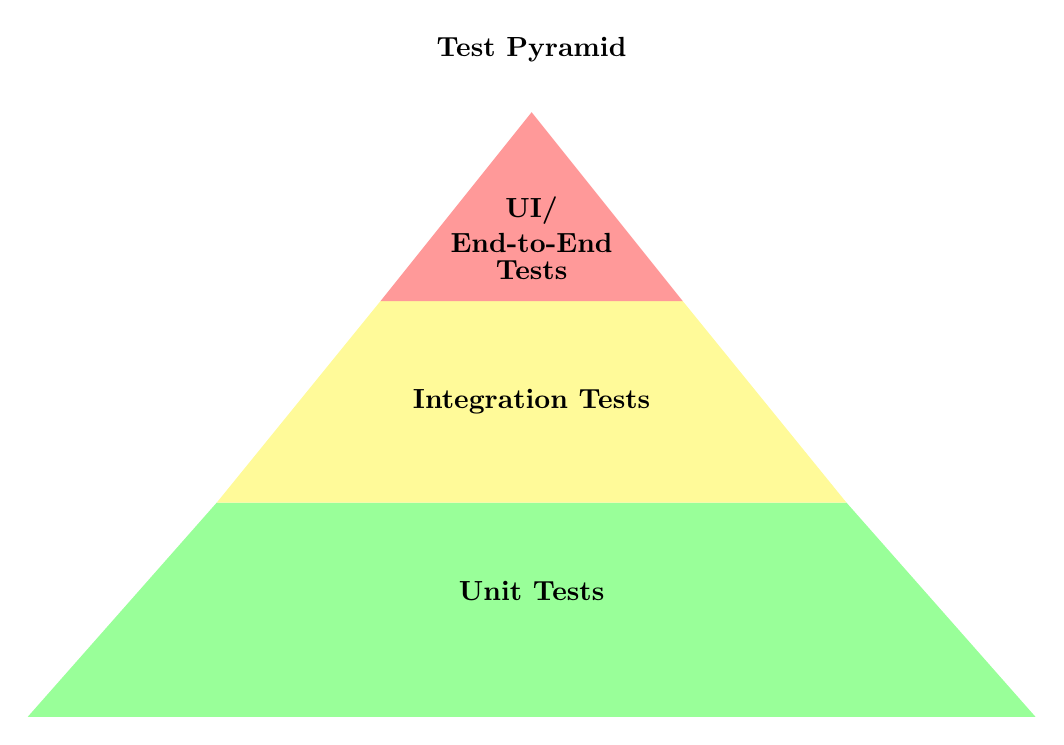
\begin{tikzpicture}[scale=1.6]
		
		% Bottom Layer: Unit Tests
		\fill[green!40] (0,0) -- (8,0) -- (6.5,1.7) -- (1.5,1.7) -- cycle;
		
		% Middle Layer: Integration Tests
		\fill[yellow!40] (1.5,1.7) -- (6.5,1.7) -- (5.2,3.3) -- (2.8,3.3) -- cycle;
		
		% Top Layer: UI Tests
		\fill[red!40] (2.8,3.3) -- (5.2,3.3) -- (4,4.8) -- cycle;

		
		% Labels
		\node at (4,1) {\textbf{Unit Tests}};
		\node at (4,2.5) {\textbf{Integration Tests}};
		\node at (4,3.8) {\shortstack{\textbf{UI/}\\\textbf{End-to-End}\\\textbf{Tests}}};

		% Title
		\node[font=\bfseries] at (4,5.3) {Test Pyramid};
		
	\end{tikzpicture}
	\caption{The Test Pyramid illustrating test distribution across levels}
	\label{fig:testpyramid}
\end{figure}


\subsection{Testing in Middleware and Distributed Systems}

\subsubsection{Specific Challenges in Testing Middleware}

Testing middleware within distributed systems presents several inherent challenges due to the complexity of distributed architectures and the abstract nature of middleware functionality. Middleware often operates across heterogeneous platforms and coordinates communication between independent software components. As Tanenbaum and van Steen emphasize, ensuring interoperability and consistent behavior across diverse systems introduces technical and architectural complexity \cite{tanenbaum2017}.
\\
\\
A core challenge is \textbf{compatibility}, as middleware must support various hardware, operating systems, network protocols, and data formats. According to Coulouris et al., this requires middleware to provide standard abstractions while hiding platform-specific details \cite{coulouris2012}. 
\\
\\
\textbf{Performance and scalability} also represent key testing concerns. Middleware must support low-latency communication and efficient resource use under variable loads. Stallings notes that poor synchronization or inefficient resource management at the middleware layer can lead to system-wide bottlenecks \cite{stallings2018}.
\\
\\
Finally, \textbf{fault tolerance} and \textbf{security} must be evaluated, particularly since middleware can be a single point of failure or a vector for attack in distributed architectures \cite{liu2009middleware}.

\subsubsection{Existing Approaches and Best Practices}

Testing middleware systems effectively requires an understanding of the system architecture and the communication patterns it supports. Burns and Wellings suggest that model-based testing is particularly suited for middleware due to its ability to describe behavior across abstraction layers \cite{burns2009real}.
\\
\\
\textbf{Integration testing} plays a vital role in evaluating message routing, service discovery, and state synchronization among components. Additionally, \textbf{system-level testing} validates functional correctness and non-functional requirements, such as real-time constraints and message reliability \cite{gorton2006software}.
\\
\\
Best practices include the use of simulation environments for performance evaluation under controlled conditions, as well as leveraging monitoring and logging tools to capture middleware-level interactions for post-test analysis. Gorton and Liu also highlight the use of profiling and benchmarking frameworks to test middleware scalability across node clusters \cite{gorton2006software}.

\subsubsection{Limitations of Current Testing Approaches for eCAL}

The enhanced Communication Abstraction Layer (eCAL) is a high-performance middleware designed for fast inter-process communication. While eCAL provides tools such as monitoring and recording utilities, a comprehensive, standardized system testing framework is not currently available.
\\
\\
Existing validation tools focus primarily on \textbf{developer-centric debugging} rather than structured system-level testing. As a result, evaluating functional correctness under distributed conditions—such as message loss, timing jitter, or node failures—requires additional tooling or custom scripts.
\\
\\
Furthermore, eCAL's support for different transport protocols (shared memory, UDP, TCP) makes performance testing across deployment contexts more difficult. Without a formal benchmarking framework, assessing eCAL's performance under various configurations is challenging. Finally, interoperability testing with other middleware remains largely undocumented in the official literature, highlighting a gap in cross-platform validation methods.

\selectlanguage{english}
\clearpage

\section{Specification}

\selectlanguage{english}
\clearpage
\section{Evaluation}

\selectlanguage{english}
\clearpage
\section{Summary}

\newpage
\printbibliography[heading=bibintoc]

\end{document}


